\documentclass[
  accentcolor=tud1c,	% Color theme for TUD corporate design
  colorbacktitle,		% Titlepage has colored background for title area
  inverttitle,			% Font color of title on titlepage is inverted
  german,
  twoside
]{tudreport}

% usepackages
\usepackage[ngerman]{babel}
\usepackage[utf8]{inputenc}
\usepackage{graphicx}
\usepackage{listings}
\usepackage{hyperref}

% define C++ listings style
\definecolor{commentgreen}{RGB}{50,127,50}
\lstloadlanguages{C++,[gnu]make}
\lstset{language=C++}
\lstset{captionpos=b}
\lstset{tabsize=3}
\lstset{breaklines=true}
\lstset{basicstyle=\ttfamily}
\lstset{columns=flexible,keywordstyle=\color{purple},stringstyle=\color{blue},commentstyle=\color{commentgreen}}
\lstset{literate=%
	{Ö}{{\"O}}1
	{Ä}{{\"A}}1
	{Ü}{{\"U}}1
	{ß}{{\ss}}2
	{ü}{{\"u}}1
	{ä}{{\"a}}1
	{ö}{{\"o}}1
	{'}{{\textquotesingle}}1
}

% intendation depth of parentheses
\parindent0pt

\title{Cheatsheet zum\linebreak[1]C/C++-Praktikum\linebreak[1] Fachgebiet Echtzeitsysteme}

\begin{document}

\maketitle

%C++:
% - Pointer, Referenzen, Doppelpointer
% - nützliche Header
% - 0, NULL <- cstddef.h
% - Schleifenkonstrukte
%   * reguläre for loop
%   * iterator-basierte for loop
%   * while-do, do-while
% - try-catch
% - Generisches Klassentemplate?
% - Syntax für Funktionspointer. Wie liest man den Typ eines Funktionspointers.
%
%C++11 (merge mit C++):
% - "nullptr"
% - foreach	(3 for schleifen varianten zeigen: normal, iterator, foreach)
% - shared_ptr
% - lambdas?
%

\chapter{Git Tutorial}
Alle notwendigen Unterlagen wie Übungsblätter, Musterlösungen etc. sind in einem Git-Repository gesammelt. Es empfiehlt sich diese zu verwenden, denn dort sind die aktuellsten Versionen verfügbar. 
Um den Zugriff über das Git-Plug-in von Eclipse einzurichten gehst du wie folgt vor:

% TODO ist per default schon da

Nun kannst du wieder in den \emph{C/C++}-View wechseln (auch möglich über \textbf{\emph{Window $\rightarrow$ Open Perspective\dots}}). Es sollte ein neues Projekt in deinem Workspace vorhanden sein, das alle Unterlagen enthält.

Neben dem Gesamtprojekt für alle Unterlagen gibt es zum Beispiel für die Musterlösung jeder Aufgabe ein eigenes Unterprojekt.

\chapter{Eclipse Tutorial}
Für alle Übungen des C/C++ Praktikums wird Eclipse zusammen mit dem C/C++ Development Tooling (CDT) und dem  GNU project C and C++ compiler (GCC) verwendet.
Wir gehen davon aus, dass der generelle Umgang mit Eclipse bereits aus der Java-Programmierung bekannt ist und nur die Unterschiede zur C++-Programmierung erläutert werden müssen.

\section{Eclipse starten}

\section{Neues Projekt anlegen}
Um ein neues Projekt anzulegen, wähle \textbf{File $\rightarrow$ New $\rightarrow$ C++ Project} im Eclipse Menü.
Gib den gewünschten Projektnamen ein und wähle \textbf{Empty Project} als Projekttyp aus.

\section{Neue Dateien zum Projekt hinzufügen}
Um eine neue Sourcecode-Datei zum Projekt hinzuzufügen, klicke mit der rechten Maustaste auf das Projekt und wähle \textbf{New $\rightarrow$ Source File}.
Gib einen Dateinamen (z.B. \emph{main.cpp}) ein und bestätige mit \textbf{Finish}. 
Verfahre analog, um Header-Dateien zu erstellen, wähle jedoch \textbf{New $\rightarrow$ Header File} im Kontextmenü.
Sourcecode-Dateien tragen in der Regel die Endung \emph{.cpp}, Header-Dateien \emph{.h} oder \emph{.hpp}.

\subsection{Neue Klassen zum Projekt hinzufügen}
Für eine Klasse kann man Header- und Sourcecode-Datei in einem Schritt erzeugen.
Wähle dazu \textbf{New $\rightarrow$ Class} im Kontext-Menü des Projekts, um den entsprechenden Wizard zu starten.
Gib den Namen und bei Bedarf den Namespace sowie weitere Informationen wie z.B. die Elternklassen ein (dazu später mehr).
Setze für die ersten Aufgaben den \textbf{virtual} Modifier des Destruktors auf \textbf{No}.


\section{Projekt kompilieren und starten}
Bevor ein C++-Programm gestartet werden kann, muss es kompiliert werden.
Im Gegensatz zu Java wird der Compiler nicht automatisch von Eclipse im Hintergrund aufgerufen, sondern muss manuell gestartet werden.
Um das aktuell offene Projekt zu kompilieren, klicke auf das \textbf{Build-}Symbol (\glqq Hammer\grqq) in der Eclipse C++ Toolbar.
Im \textbf{Console-}Fenster unten werden Compiler-Meldungen und eventuelle Fehler während des Erstellungsprozesses angezeigt.

Öffne zum Starten des Programms das Kontextmenü des Projekts und wähle \textbf{Run As$\rightarrow$ Local C/C++ Application }.
Danach kannst du zum Starten den grünen Run-Knopf benutzen.

\subsection{Projekt debuggen}
Du kannst dein Programm auch im Debug-Modus laufen lassen, um dir Schritt für Schritt den Ablauf anzusehen und mögliche Fehler zu finden.
Zum Debuggen wählst du (wie auch bei Java) den Debug-Knopf (\glqq Käfer\grqq) und Eclipse wird automatisch in die Debug-Perspektive wechseln.


\section{Eclipse Shortcuts}
\begin{tabular}{l|l|p{11.5cm}}
	Ctrl+Space & Autocomplete &
	Anzeige von Vervollständigungshinweisen (z.B. nach \emph{std::} oder \emph{main})
	\\\hline
	Alt+Shift+R & Rename &
	Umbennenen von Variablen, Funktionen, Klassen, \dots
	\\\hline
	Ctrl+N & New &
	Anlegen neuer Ressourcen (Dateien, Projekte, \dots)
	\\\hline
	Ctrl+Tab & Header$\leftrightarrow$Source &
	Wechsel zwischen der Header- und der Implementierungsdatei
	\\\hline
	Ctrl+Click/F3 & Go to &
	Navigiert zu der Definition eines Elements (Funktion, Klasse, Variable, \dots)
	\\\hline
	Ctrl+B & Build &
	Startet den Buildprozess (Aufruf von Compiler und Linker)
\end{tabular}

\section{Häufige Compiler-Fehlermeldungen des gcc}

\begin{verbatim}
error: expected ';' before ...
\end{verbatim}

Dies bedeutet, dass in der Zeile davor ein \textbf{;} vergessen wurde.
Allgemein beziehen sich Fehlermeldungen \textbf{expected ... before ...} häufig auf die Zeile \textbf{vor} dem markierten Statement.
Beachte, dass \emph{die Zeile davor} auch die letzte Zeile einer eingebundenen Header-Datei sein kann. Beispiel:

\begin{lstlisting}
#include "main.h"
int main() {
	...
}
\end{lstlisting}

Falls im Header \emph{main.h} in der letzten Zeile ein Semikolon fehlt, wird der Compiler die Fehlermeldung trotzdem auf die Zeile \textbf{int main() \{} beziehen!!

\begin{verbatim}
error: invalid conversion from <A> to <B>.
\end{verbatim}

Dies bedeutet, dass der Compiler an der entsprechenden Stelle einen Ausdruck vom Typ \emph{B} erwartet, im Code jedoch ein Ausdruck vom Typ \emph{A} angegeben wurde. Insbesondere bei verschachtelten Typen sowie (später vorgestellten) Zeigern und Templates kann die Fehlermeldung sehr lang werden. In so einem Fall lohnt es sich, den Ausdruck in mehrere Teilausdrücke aufzubrechen und die Teilergebnisse durch temporäre Variablen weiterzureichen.

\begin{verbatim}
undefined reference to ...
\end{verbatim}

Dies bedeutet, dass das Programm zwar korrekt kompiliert wurde, der Linker aber die Definition des entsprechenden Bezeichners nicht finden kann.
Das kann passieren, wenn man dem Compiler durch einen Prototypen mitteilt, dass eine bestimmte Funktion existiert (\textbf{deklariert}), diese aber nirgendwo tatsächlich \textbf{definiert}.
Überprüfe in diesem Fall, ob der Bezeichner tatsächlich definiert wurde und ob die Signatur der Definition mit dem Prototypen übereinstimmt.



\chapter{C++}
\section{Minimalprogramm}


\subsection{Primitive Datentypen}
Die primitiven Datentypen in C++ sind ähnlich denen in Java.
Allerdings sind alle Ganzzahl-Typen in C++ sowohl mit als auch ohne Vorzeichen verfügbar.
Standardmäßig sind Zahlen vorzeichenbehaftet.
Mittels \textbf{unsigned} kann man vorzeichenlose Variablen deklarieren.
Durch das freie Vorzeichenbit kann ein größerer positiver Wertebereich dargestellt werden.

\begin{lstlisting}
 	int i; // signed int, -2147483648 to +2147483647 on 32-bit machine
	unsigned int ui; // unsigned int, 0 to 4294967295 on 32-bit machine
	// unsigned double d; // not possible
\end{lstlisting}

Eine andere Besonderheit von C++ ist, dass Ganzzahlwerte implizit in Boolesche Werte (Typ: \emph{bool}) umgewandelt werden.
Alles ungleich 0 wird als \textbf{true} gewertet, 0 als \textbf{false}.
Somit können Ganzzahlen direkt in Bedingungen ausgewertet werden:

\begin{lstlisting}
 	int n = 5;
 	// loop which runs until n is 0
 	while(n--) { // post-decrement n, i.e. decrement n but return previous value
  		cout << n << endl;
 	}

	// output: 4 3 2 1 0
\end{lstlisting}

\section{C++11}



\chapter{Mikrocontroller}

\begin{center}
	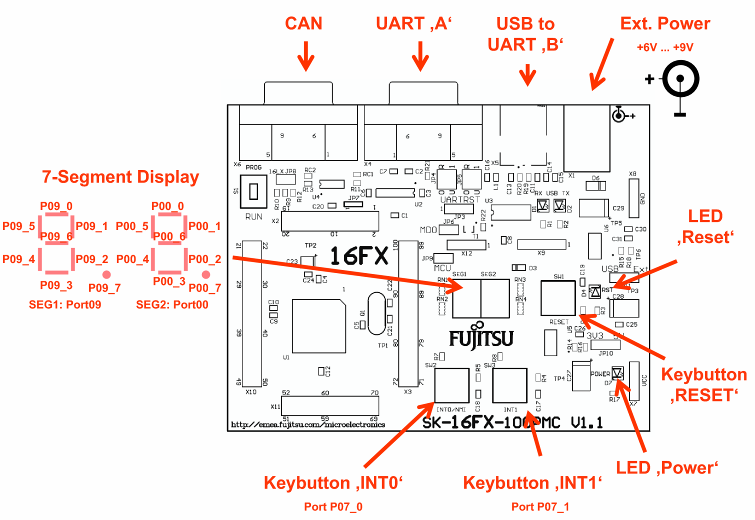
\includegraphics[width=0.6\textwidth]{figures/starterkit.png}
\end{center}

%\section{Flashen und Ausführen}
%Voraussetzung: Das Board ist über USB korrekt an dem Rechner angeschlossen.
%\begin{enumerate}
%	\item Schiebeschalter auf \textbf{PROG} stellen
%	\item Build in Eclipse und Flashen mit FLASHly
%	\item Schiebeschalter auf \textbf{RUN} stellen
%	\item \textbf{RESET} Button betätigen
%\end{enumerate}

\section{C}
\subsection{Minimalprogramm}
Folgendes Programm läuft bleibt unendlich lange in der for-Schleife und führt bei jedem Durchgang eine Warteoperation durch.
Die Include-Anweisung ist notwendig, um das Programm auf dem Mikrocontroller zu verwenden.
Es bietet Zugang zur Hardware, als auch Systemfunktionen wie zum Beispiel die Warteoperation.
% TODO wozu NOP überhaupt?
\begin{lstlisting}
#include "mb96348hs.h"
void main(void) {
	for (;;) {
		__wait_nop();
	}
}
\end{lstlisting}
% - generisches Programm: main loop, Variablen müssen am Anfang des Scopes deklariert werden
% - Ansteuerung 7-Segment-Anzeige
% - Auslesen Taster
% - Auslesen Poti
% - Ansteuerung LCD

\end{document}
